\chapter{Communicate with the robot via controller module}
\section{Robot interface command}
\begin{itemize}
	\item[--] GotoXYZ
	\item[--] MoveToDest
	\item[--] ClickUp
	\item[--] ClickDown
\end{itemize}

\section{Control robot synchronized with testing script}
\subsection{System implementation}
Whole system class diagram
    \begin{figure}[H]
		\centering
		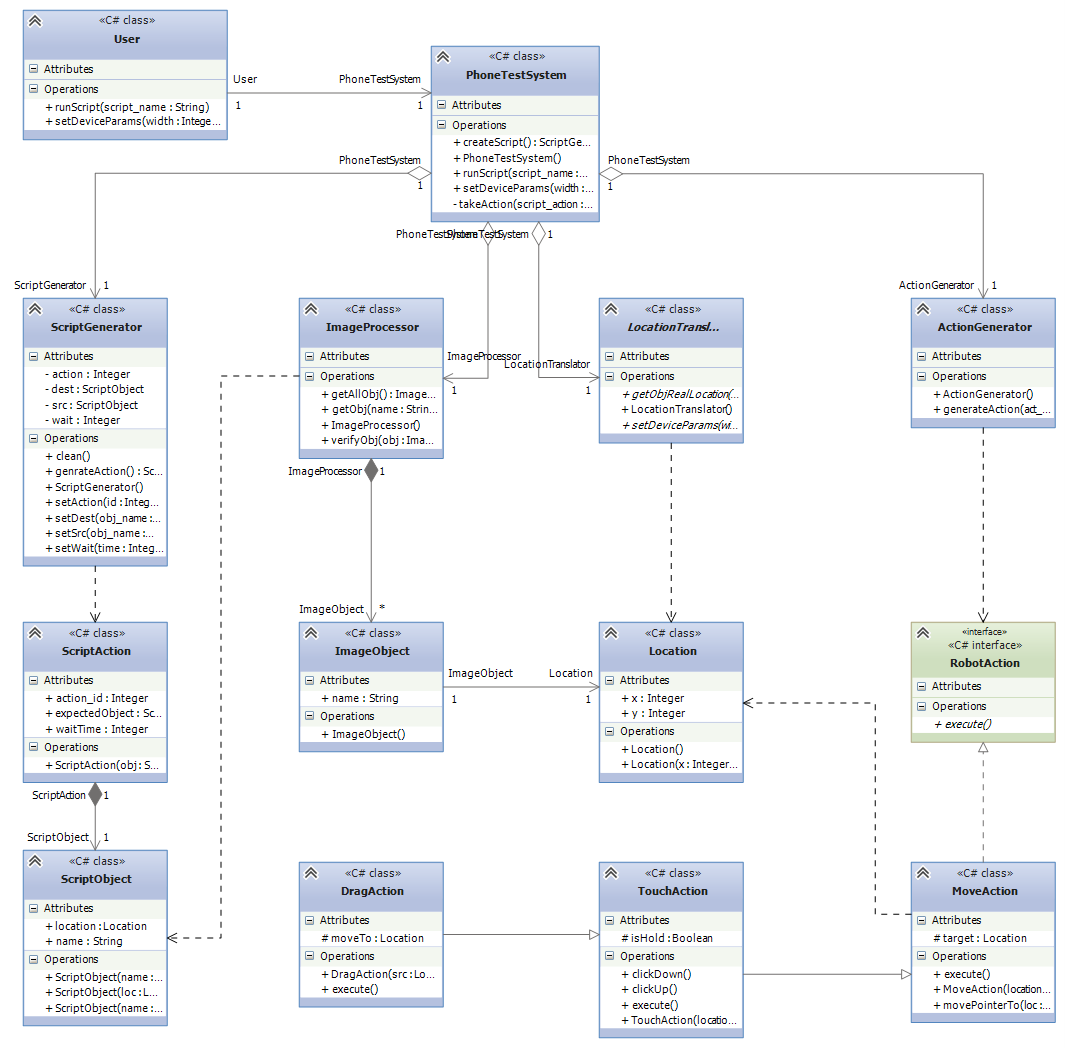
\includegraphics[scale=0.55]{Chapters/Fig/class_diagram.png}
		\caption{System class diagram}
		\label{fig:class_diagram}
	\end{figure}

Main components of the system
	\begin{figure}[H]
		\centering
		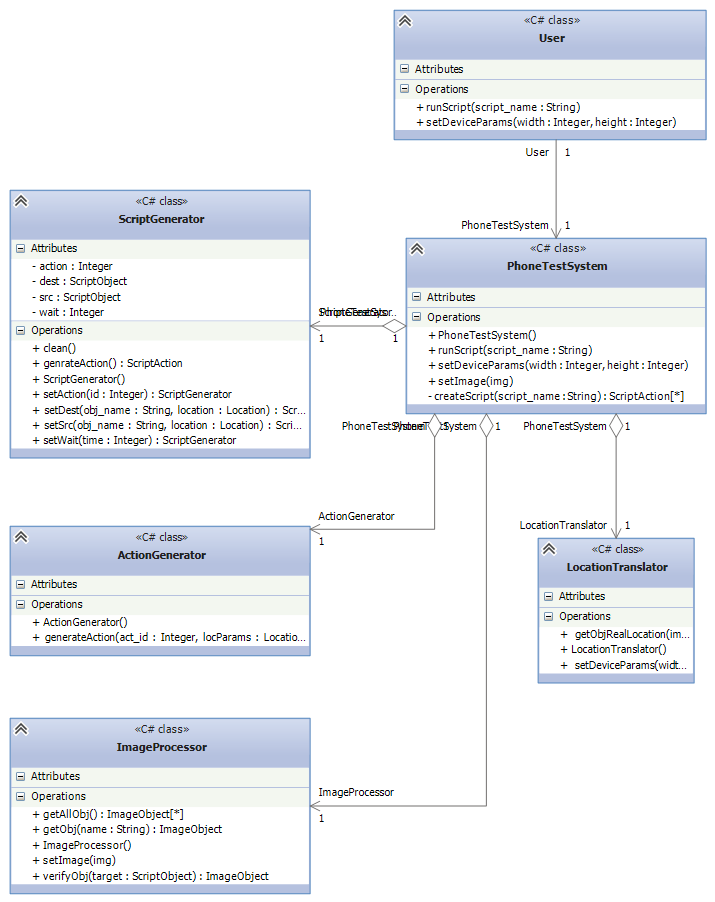
\includegraphics[scale=0.75]{Chapters/Fig/main_class.png}
		\caption{System main components}
		\label{fig:main_class}
	\end{figure}

Script Generator structure
	\begin{figure}[H]
		\centering
		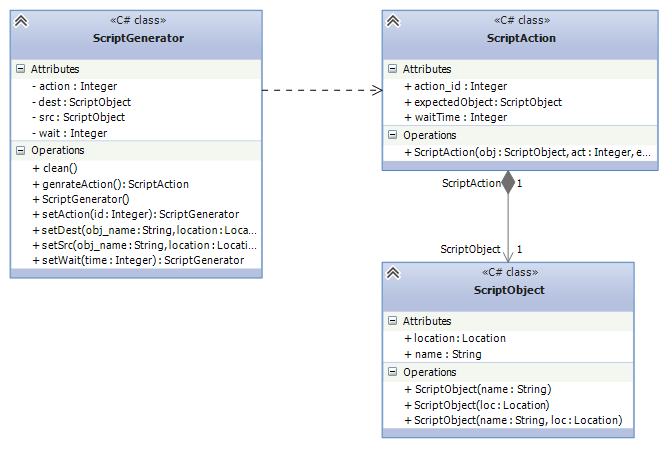
\includegraphics[scale=0.75]{Chapters/Fig/script_gen.png}
		\caption{Script Generator structure}
		\label{fig:script_gen}
	\end{figure}

Image Processor structure
	\begin{figure}[H]
		\centering
		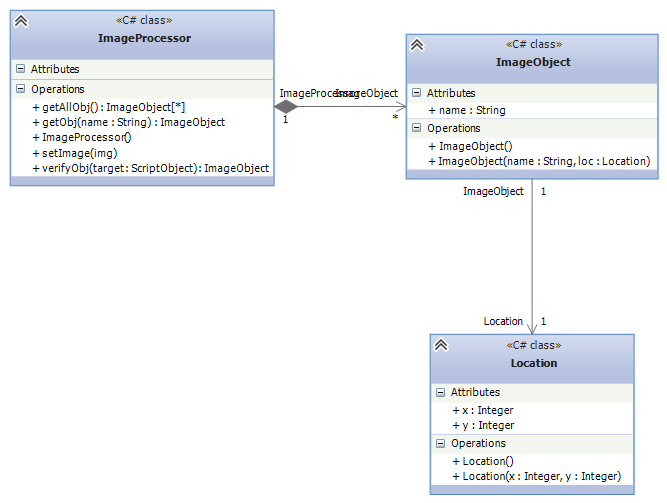
\includegraphics[scale=0.75]{Chapters/Fig/img_processor.png}
		\caption{Image Processor structure}
		\label{fig:img_processor}
	\end{figure}

Action Generator structure
	\begin{figure}[H]
		\centering
		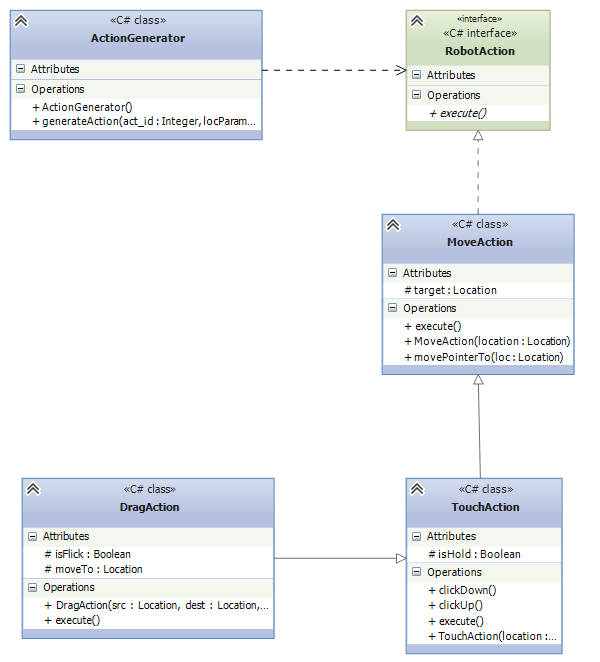
\includegraphics[scale=0.75]{Chapters/Fig/act_gen.png}
		\caption{Action Generator structure}
		\label{fig:act_gen}
	\end{figure}

